\heading{理论力学-24春-期中}

\begin{question}[离心调速器]
如图，离心调速器以恒定角速度 $\omega$ 转动，$A$ 和 $B$ 的质量均为 $m$，$C$ 的质量为 $M$，各轻杆的长度均为 $L$。用虚功原理求系统平衡时的张角 $\varphi$。

\begin{center}
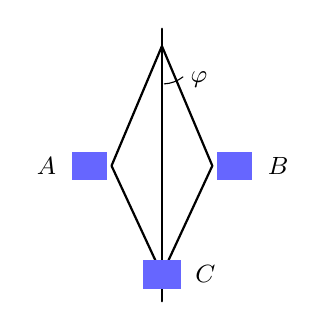
\begin{tikzpicture}[x=1cm,y=1cm,line cap=round,line join=round,font=\small]
  \coordinate (T) at (0,1.86);
  \coordinate (A1) at (-0.84,0.34);
  \coordinate (B1) at (0.84,0.34);
  \coordinate (C1) at (0,-1.04);
  \draw[line width=0.8pt] (0,2.08) -- (0,-1.38);
  \draw[line width=0.8pt] (T)--(-0.64,0.34)--(C1)--(0.64,0.34)--cycle;
  \fill[blue!60] (-1.14,0.16) rectangle (-0.70,0.52);
  \fill[blue!60] (0.70,0.16) rectangle (1.14,0.52);
  \fill[blue!60] (-0.24,-1.22) rectangle (0.24,-0.86);
  \node[left] at (-1.22,0.34) {$A$};
  \node[right] at (1.22,0.34) {$B$};
  \node[right] at (0.30,-1.04) {$C$};
  \draw (0.03,1.38) arc[start angle=-87,end angle=-52,radius=0.42];
  \node[right] at (0.24,1.44) {$\varphi$};
\end{tikzpicture}

{\small 题 1 示意图}
\end{center}

\begin{solution}
在随调速器匀速转动的参考系中使用有效势能。设两侧小球到转轴的距离为
\[
  r=L\sin\varphi.
\]
以顶部铰点为高度零点，两个小球的高度均为 $-L\cos\varphi$，滑块 $C$ 的高度为 $-2L\cos\varphi$。因此重力势能为
\[
  V_g=-2mgL\cos\varphi-2MgL\cos\varphi.
\]
两个小球的离心势能为
\[
  V_c=-2\cdot\frac12m\omega^2r^2=-m\omega^2L^2\sin^2\varphi.
\]
有效势能
\[
  V_{\mathrm{eff}}=-2(m+M)gL\cos\varphi-m\omega^2L^2\sin^2\varphi.
\]
平衡条件为
\[
  \frac{\dd V_{\mathrm{eff}}}{\dd\varphi}=0.
\]
除去 $\sin\varphi=0$ 的退化位置，得
\[
  2(m+M)gL-2m\omega^2L^2\cos\varphi=0.
\]
故
\[
  \boxed{\cos\varphi=\frac{(m+M)g}{m\omega^2L}}.
\]
存在非零张角平衡要求
\[
  \boxed{\omega^2\ge \frac{(m+M)g}{mL}}.
\]


\medskip
\textbf{虚功写法：}令 $\varphi$ 作虚位移 $\delta\varphi$。两球的高度变化为
\[
  \delta z_A=\delta z_B=L\sin\varphi\,\delta\varphi,
\]
滑块 $C$ 的高度变化为
\[
  \delta z_C=2L\sin\varphi\,\delta\varphi.
\]
重力虚功为
\[
  \delta W_g=-2mgL\sin\varphi\,\delta\varphi
  -2MgL\sin\varphi\,\delta\varphi.
\]
离心力只作用于两侧小球，每个小球的离心力为 $m\omega^2L\sin\varphi$，径向位移为 $L\cos\varphi\delta\varphi$，所以
\[
  \delta W_c=2m\omega^2L^2\sin\varphi\cos\varphi\,\delta\varphi.
\]
由 $\delta W_g+\delta W_c=0$，除去 $\sin\varphi=0$ 后即得前述平衡条件。
\end{solution}
\end{question}

\begin{question}[摆长线性变化的单摆]
设单摆的摆长满足
\[
  l(t)=l_0-vt,
\]
其中 $v$ 为常量，且 $t<l_0/v$。使用拉格朗日方法求摆角 $\varphi$ 所满足的微分方程。

\begin{solution}
摆长 $l(t)=l_0-vt$ 是给定函数，不作为广义坐标。摆角为 $\varphi$ 时，动能和势能可写为
\[
  T=\frac12m\left(\dot l^2+l^2\dot\varphi^2\right),
  \qquad
  V=-mgl\cos\varphi.
\]
与 $\varphi$ 有关的拉格朗日量为
\[
  L=\frac12ml^2\dot\varphi^2+mgl\cos\varphi.
\]
拉格朗日方程给出
\[
  \frac{\dd}{\dd t}\left(ml^2\dot\varphi\right)+mgl\sin\varphi=0.
\]
因此
\[
  l^2\ddot\varphi+2l\dot l\dot\varphi+gl\sin\varphi=0.
\]
代入 $l=l_0-vt$、$\dot l=-v$，得
\[
  \boxed{\ddot\varphi-\frac{2v}{l_0-vt}\dot\varphi
  +\frac{g}{l_0-vt}\sin\varphi=0}.
\]


\medskip
\textbf{方程检查：}虽然 $\dot l^2$ 出现在动能中，但它不含 $\varphi$ 与 $\dot\varphi$，所以不会进入 $\varphi$ 的 Euler--Lagrange 方程。由于 $l(t)$ 显含时间，系统机械能一般不守恒；外部收放摆线会对摆球作功。小角度近似下方程变为
\[
  \ddot\varphi-\frac{2v}{l_0-vt}\dot\varphi
  +\frac{g}{l_0-vt}\varphi=0,
\]
其中中间项来自角动量 $ml^2\dot\varphi$ 中随时间改变的 $l^2$。


\medskip
如果从极坐标速度公式出发，质点速度平方为
\[
  v_p^2=\dot l^2+l^2\dot\varphi^2.
\]
这里没有 $2\dot l l\dot\varphi$ 交叉项，因为径向单位矢量与切向单位矢量正交。势能若取最低点为零，可写成 $mgl(1-\cos\varphi)$；与本文采用的 $-mgl\cos\varphi$ 只差一个显含时间的函数 $mgl(t)$，不会改变 $\varphi$ 方程。
\end{solution}
\end{question}

\begin{question}[椭圆摆]
考虑如图所示的椭圆摆。滑块 $A$ 的位置坐标为 $x$，摆长为 $L$，摆角为 $\theta$，滑块 $A$ 和摆球 $B$ 的质量均为 $m$。初始条件为 $t=0$ 时 $\theta=\theta_0$，$x=0$。

\begin{center}
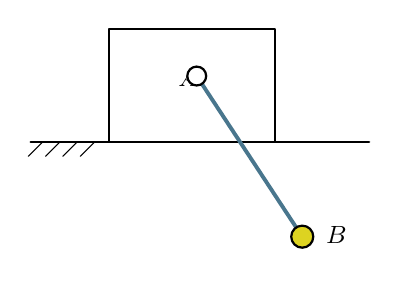
\begin{tikzpicture}[x=1cm,y=1cm,line cap=round,line join=round,font=\small]
  \draw[line width=0.8pt] (-2.15,0) -- (2.15,0);
  \foreach \x in {-2.00,-1.78,...,-1.18} {\draw[thin] (\x,0) -- (\x-0.18,-0.18);} 
  \draw[line width=0.8pt] (-1.15,0) rectangle (0.95,1.44);
  \node at (-0.15,0.82) {$A$};
  \coordinate (P) at (-0.04,0.84);
  \coordinate (Q) at (1.30,-1.20);
  \draw[line width=1.4pt,cyan!50!black] (P) -- (Q);
  \draw[line width=0.8pt,fill=white] (P) circle (0.12);
  \draw[line width=0.8pt,fill=yellow!85!black] (Q) circle (0.14);
  \node[right] at (1.48,-1.18) {$B$};
\end{tikzpicture}

{\small 题 3 示意图}
\end{center}

\begin{enumerate}
  \item 用拉格朗日方法求系统的运动；
  \item 求系统的初积分。
\end{enumerate}

\begin{solution}
滑块 $A$ 的坐标为 $x$，摆球 $B$ 的坐标为
\[
  X_B=x+L\sin\theta,
  \qquad
  Y_B=-L\cos\theta .
\]
两者质量均为 $m$，故
\[
  T=\frac12m\dot x^2+\frac12m\left[(\dot x+L\cos\theta\dot\theta)^2
  +(L\sin\theta\dot\theta)^2\right].
\]
即
\[
  T=m\dot x^2+mL\cos\theta\dot x\dot\theta+\frac12mL^2\dot\theta^2.
\]
势能为
\[
  V=-mgL\cos\theta.
\]
\begin{enumerate}
  \item 拉格朗日量为
  \[
    L=T-V=m\dot x^2+mL\cos\theta\dot x\dot\theta
    +\frac12mL^2\dot\theta^2+mgL\cos\theta.
  \]
  拉格朗日方程为
  \[
    2\ddot x+L\left(\cos\theta\ddot\theta-\sin\theta\dot\theta^2\right)=0,
  \]
  \[
    L\ddot\theta+\cos\theta\ddot x+g\sin\theta=0.
  \]
  \item 由于 $x$ 是循环坐标，
  \[
    p_x=2m\dot x+mL\cos\theta\dot\theta=P
  \]
  为初积分。能量也守恒：
  \[
    E=m\dot x^2+mL\cos\theta\dot x\dot\theta+\frac12mL^2\dot\theta^2-mgL\cos\theta.
  \]
  若初始总水平动量为零，则
  \[
    \dot x=-\frac L2\cos\theta\dot\theta,
  \]
  从而可将运动化为 $\theta$ 的一维问题。
\end{enumerate}


\medskip
\textbf{化为一维问题：}若初始时系统水平总动量为零，则循环坐标给出 $P=0$，即
\[
  2\dot x+L\cos\theta\dot\theta=0.
\]
将其代入能量，可得
\[
  E=mL^2\left(\frac12-\frac14\cos^2\theta\right)\dot\theta^2-mgL\cos\theta.
\]
于是 $\theta(t)$ 可由一阶方程求出，随后再由
\[
  \dot x=-\frac L2\cos\theta\dot\theta
\]
积分得到 $x(t)$。这说明系统的两个初积分足以把运动降为求积问题。
\end{solution}
\end{question}

\begin{question}[圆盘作无滑动滚动]
在 $xOy$ 平面上，一个质量为 $m$、半径为 $R$ 的均匀圆盘作无滑动滚动，并满足约束：盘心到接触点的连线始终垂直于平面。
\begin{enumerate}
  \item 分析系统的自由度，并选取合适的广义坐标；
  \item 写出系统的拉格朗日量 $L$，并用拉格朗日乘子法求系统的运动微分方程。
\end{enumerate}

\begin{solution}
圆盘始终竖直，故可取盘心坐标 $(x,y)$、圆盘前进方向角 $\varphi$ 和自转角 $\psi$ 为广义坐标。其中 $\varphi$ 是圆盘平面法线在 $xOy$ 平面内的方位角，$\psi$ 是绕圆盘对称轴的自转角。

均匀圆盘关于对称轴的转动惯量为
\[
  I_3=\frac12mR^2,
\]
关于任一直径的转动惯量为
\[
  I_1=\frac14mR^2.
\]
因此无约束形式的动能为
\[
  T=\frac12m(\dot x^2+\dot y^2)
    +\frac12 I_3\dot\psi^2+\frac12 I_1\dot\varphi^2
  =\frac12m(\dot x^2+\dot y^2)
    +\frac14mR^2\dot\psi^2+\frac18mR^2\dot\varphi^2 .
\]
势能为常数，可取为零，故 $L=T$。

纯滚动约束是接触点瞬时速度为零，即
\[
  \dot x=R\dot\psi\cos\varphi,
  \qquad
  \dot y=R\dot\psi\sin\varphi .
\]
这两个约束不可积分为仅含坐标的方程，因此系统有 $4$ 个广义坐标、$2$ 个独立非完整约束，运动自由度为
\ansmath{4-2=2.}

用拉格朗日乘子 $\lambda_1,\lambda_2$ 写约束为
\[
  \dot x-R\dot\psi\cos\varphi=0,
  \qquad
  \dot y-R\dot\psi\sin\varphi=0 .
\]
Lagrange--d'Alembert 方程为
\[
  m\ddot x=\lambda_1,
  \qquad
  m\ddot y=\lambda_2,
\]
\[
  \frac14mR^2\ddot\psi
  =-R(\lambda_1\cos\varphi+\lambda_2\sin\varphi),
  \qquad
  \frac14mR^2\ddot\varphi=0.
\]
连同两个约束方程共同决定系统运动。由最后一式可知
\ansmath{\dot\varphi=\text{const.}}
即圆盘前进方向的角速度保持不变。若先代入约束，则约化拉格朗日量为
\[
  L_{\mathrm{red} }
  =\frac34mR^2\dot\psi^2+\frac18mR^2\dot\varphi^2,
\]
但要强调：由于约束是非完整约束，严格推导运动方程应使用上面的乘子法，而不能把非完整约束当作完整约束直接变分。
\end{solution}

\end{question}

\begin{question}[四自由度系统的小振动]
一个自由度为 $4$ 的理想、完整且稳定约束的保守力学体系，其广义坐标为 $q_\alpha$（$\alpha=1,2,3,4$）。相应势能与动能二次型的系数矩阵分别为（其中 $\omega_0>0$）
\[
  \mathbf{V}=\begin{pmatrix}
    1&0&0&0\\
    0&1&0&0\\
    0&0&2&-2\\
    0&0&-2&3
  \end{pmatrix}\omega_0^2,
  \qquad
  \mathbf{T}=\begin{pmatrix}
    1&0&0&0\\
    0&1&0&0\\
    0&0&1&-1\\
    0&0&-1&2
  \end{pmatrix}.
\]
\begin{enumerate}
  \item 求体系的小振动解，并根据求得的本征矢量判断哪些广义坐标已经是简正坐标；
  \item 找出全部简正坐标，并求其小振动解；
  \item 在求得的 $4$ 个本征频率中，哪些是简并的？简并度各是多少？
\end{enumerate}

\begin{solution}
小振动方程可写为
\[
  \mathbf T\ddot{\boldsymbol q}+\omega_0^2\mathbf V\boldsymbol q=0.
\]
令
\[
  \boldsymbol q=\boldsymbol a\ee^{\ii\omega t},
  \qquad
  \lambda=\frac{\omega^2}{\omega_0^2},
\]
得到广义本征值问题
\[
  (\mathbf V-\lambda\mathbf T)\boldsymbol a=0.
\]
直接计算
\[
  \det(\mathbf V-\lambda\mathbf T)=(\lambda-1)^3(\lambda-2).
\]
因此本征频率为
\ansmath{\omega=\omega_0\quad(\text{三重}),\qquad \omega=\sqrt2\,\omega_0\quad(\text{单重}).}
对应的本征矢量可取为
\[
  \lambda=1:
  \quad
  (1,0,0,0)^{\mathsf T},\quad
  (0,1,0,0)^{\mathsf T},\quad
  (0,0,1,1)^{\mathsf T},
\]
\[
  \lambda=2:
  \quad
  (0,0,1,0)^{\mathsf T}.
\]
\begin{enumerate}
  \item 由前两个本征矢量可见，$q_1$ 与 $q_2$ 本身已经是简正坐标；$q_3,q_4$ 的组合还需要重新选取。
  \item 按
  \[
    \boldsymbol q=Q_1(1,0,0,0)^{\mathsf T}
    +Q_2(0,1,0,0)^{\mathsf T}
    +Q_3(0,0,1,1)^{\mathsf T}
    +Q_4(0,0,1,0)^{\mathsf T}
  \]
  展开，可得
  \[
    q_1=Q_1,
    \qquad
    q_2=Q_2,
    \qquad
    q_3=Q_3+Q_4,
    \qquad
    q_4=Q_3.
  \]
  因而一组简正坐标为
  \ansmath{Q_1=q_1,
    \qquad Q_2=q_2,
    \qquad Q_3=q_4,
    \qquad Q_4=q_3-q_4.}
  它们满足
  \[
    \ddot Q_1+\omega_0^2Q_1=0,
    \quad
    \ddot Q_2+\omega_0^2Q_2=0,
    \quad
    \ddot Q_3+\omega_0^2Q_3=0,
  \]
  \[
    \ddot Q_4+2\omega_0^2Q_4=0.
  \]
  所以
  \[
    Q_j=A_j\cos(\omega_jt)+B_j\sin(\omega_jt),
  \]
  其中 $\omega_1=\omega_2=\omega_3=\omega_0$，$\omega_4=\sqrt2\omega_0$。
  \item 简并频率为 $\omega_0$，简并度为 $3$；频率 $\sqrt2\omega_0$ 不简并。
\end{enumerate}
\end{solution}

\end{question}

\begin{question}[等时摆曲线]
一般单摆的运动周期依赖于振幅。若要求物体在任意振幅下都作简谐运动，问它应沿怎样的曲线运动？请用拉格朗日方法求解。

\begin{solution}
设曲线上从最低点量起的弧长为 $s$，高度为 $y(s)$。质点沿曲线运动时
\[
  L=\frac12m\dot s^2-mgy(s).
\]
若要求任意振幅下运动都为简谐振动，则应有
\[
  \ddot s+\omega^2 s=0.
\]
与 Euler--Lagrange 方程
\[
  m\ddot s+mg\frac{\dd y}{\dd s}=0
\]
比较，得到
\[
  \frac{\dd y}{\dd s}=\frac{\omega^2}{g}s,
  \qquad
  y=\frac{\omega^2}{2g}s^2.
\]
这说明高度必须是弧长的二次函数。

满足这一性质的曲线是摆线。令生成圆半径为 $a$，摆线可写为
\[
  x=a(\theta+\sin\theta),
  \qquad
  y=a(1-\cos\theta).
\]
从最低点量起的弧长为
\[
  s=4a\sin\frac\theta2,
\]
而高度为
\[
  y=2a\sin^2\frac\theta2=\frac{s^2}{8a}.
\]
于是运动方程为
\[
  \ddot s+\frac{g}{4a}s=0,
\]
周期为
\ansmath{T=4\pi\sqrt{\frac ag},}
与振幅无关。因此所求等时摆曲线为
\ansmath{x=a(\theta+\sin\theta),\qquad y=a(1-\cos\theta)}
或与之平移、反向后的同一摆线。


\medskip
\textbf{几何核查：}对摆线参数式
\[
  x=a(\theta+\sin\theta),\qquad y=a(1-\cos\theta),
\]
有
\[
  \frac{\dd x}{\dd\theta}=a(1+\cos\theta),
  \qquad
  \frac{\dd y}{\dd\theta}=a\sin\theta.
\]
故弧长微元为
\[
  \dd s=a\sqrt{(1+\cos\theta)^2+\sin^2\theta}\,\dd\theta
  =2a\cos\frac\theta2\,\dd\theta,
\]
从最低点起积分得到 $s=4a\sin(\theta/2)$。代回高度 $y=2a\sin^2(\theta/2)$，确有 $y=s^2/(8a)$，因此运动方程严格线性，而不是小振幅近似线性。
\end{solution}

\end{question}

\begin{question}[三种宇宙速度]
求第一、第二和第三宇宙速度，并给出推导过程。

可取地球质量 $M_\oplus$、地球半径 $R_\oplus$、太阳质量 $M_\odot$ 和日地距离 $R_E$ 为已知量；数值计算时可使用 $g=9.81\,\mathrm{m/s^2}$。

\begin{solution}
以下按通常定义，三种宇宙速度均指从地球表面附近发射、忽略大气阻力和地球自转修正时的速度。

第一宇宙速度是近地圆轨道速度，由万有引力提供向心力：
\[
  \frac{GM_\oplus m}{R_\oplus^2}=m\frac{v_1^2}{R_\oplus}.
\]
故
\ansmath{v_1=\sqrt{\frac{GM_\oplus}{R_\oplus}}=\sqrt{gR_\oplus}\approx 7.91\,\mathrm{km/s}.}

第二宇宙速度是从地球表面逃逸到无穷远且剩余速度为零的速度。由能量守恒
\[
  \frac12mv_2^2-\frac{GM_\oplus m}{R_\oplus}=0,
\]
得
\ansmath{v_2=\sqrt{\frac{2GM_\oplus}{R_\oplus}}=\sqrt2\,v_1\approx 11.2\,\mathrm{km/s}.}

第三宇宙速度要求飞行器最终逃离太阳系。地球绕太阳的公转速度为
\[
  v_E=\sqrt{\frac{GM_\odot}{R_E}},
\]
其中 $R_E$ 为日地距离。飞行器在地球轨道处相对太阳逃逸所需的日心速度为
\[
  v_{\mathrm{esc},\odot}=\sqrt{\frac{2GM_\odot}{R_E}}=\sqrt2\,v_E.
\]
若沿地球公转方向发射，需要的地球逃逸后的双曲线剩余速度最小，为
\[
  v_\infty=(\sqrt2-1)v_E.
\]
从地面发射时还必须克服地球引力，因此
\[
  v_3^2=v_2^2+v_\infty^2.
\]
于是
\ansmath{v_3=\sqrt{v_2^2+\bigl[(\sqrt2-1)v_E\bigr]^2}\approx 16.7\,\mathrm{km/s}.}
这里 $v_E\approx29.8\,\mathrm{km/s}$。题目给出的月球、太阳半径和博雅塔高度等数据不进入标准三种宇宙速度的主导计算；若要求从其他天体表面发射，只需把相应的 $M,R$ 代入同样的逃逸速度公式。


\medskip
\textbf{数值计算：}第一、第二宇宙速度只涉及地球的 $M_\oplus,R_\oplus$。第三宇宙速度还需要日地距离 $R_E$，因为必须先比较地球公转速度与太阳逃逸速度。取日地平均距离
\[
  R_E=1\,\mathrm{AU},\qquad v_E\simeq29.8\,\mathrm{km/s}.
\]
最小第三宇宙速度要求从地球出发时沿地球公转方向获得双曲剩余速度；若方向不沿公转方向，所需地面速度会更大。
\end{solution}

\end{question}

\begin{question}[Yukawa 势中的稳定圆轨道]
电子在势场
\[
  V(r)=-\frac{k\ee^{-\alpha_0 r}}{r}
\]
中运动。分析稳定圆轨道应满足的条件。

\begin{solution}
有效势能为
\[
  V_{\mathrm{eff}}(r)=\frac{J^2}{2mr^2}-\frac{k\ee^{-\alpha_0 r}}{r}.
\]
圆轨道半径为 $a$ 时，
\[
  V_{\mathrm{eff}}'(a)=0.
\]
稳定性要求
\[
  V_{\mathrm{eff}}''(a)>0.
\]
计算并利用圆轨道条件消去 $J$，得
\[
  V_{\mathrm{eff}}''(a)=\frac{k\ee^{-\alpha_0a}}{a^3}
  \left(1+\alpha_0a-\alpha_0^2a^2\right).
\]
因此稳定圆轨道满足
\[
  \boxed{1+\alpha_0a-\alpha_0^2a^2>0},
\]
即
\[
  \boxed{0<\alpha_0a<\frac{1+\sqrt5}{2}}.
\]


\medskip
\textbf{关键步骤：}若写成径向扰动形式，令 $r=a+\rho$，则
\[
  m\ddot\rho+V_{\mathrm{eff}}''(a)\rho=0.
\]
所以稳定圆轨道不仅要求存在圆轨道，即 $V_{\mathrm{eff}}'(a)=0$，还要求 $V_{\mathrm{eff}}''(a)>0$。当
\[
  \alpha_0a=\frac{1+\sqrt5}{2}
\]
时为临界情形，二次项消失，需要保留更高阶项；超过此值时有效势在圆轨道半径处为极大值，径向扰动会增大。


\medskip
圆轨道的角速度也可写出。由 $J=ma^2\dot\varphi$ 和圆轨道条件得
\[
  \dot\varphi^2=\frac{k\ee^{-\alpha_0a}(1+\alpha_0a)}{ma^3}.
\]
若径向扰动稳定，则径向振动频率为
\[
  \omega_r^2=\frac{k\ee^{-\alpha_0a}}{ma^3}
  (1+\alpha_0a-\alpha_0^2a^2).
\]
注意 $\omega_r$ 与圆周角速度一般不相等，因此轨道微扰后通常不再闭合。
\end{solution}
\end{question}
